\documentclass[tikz]{standalone}

\usetikzlibrary{calc}

\tikzset{signal/.style={%
  ->,
  very thick,
  >=latex,
  rounded corners,
  }
}

\tikzset{block/.style={%
  inner sep=2mm,
  anchor=center,
  rounded corners,
  very thick,
  draw,
  }
}

\tikzset{block diagram/.style={every path/.style={signal},every node/.style={block,draw=none}}}

\begin{document}

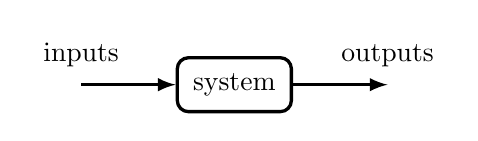
\begin{tikzpicture}[block diagram]
  
  \node (system) [block] {system};
  
  \draw ($(system.west)-(1.2cm,0)$) -- node[pos=0,anchor=south] {inputs} (system);
  \draw (system) -- node[pos=1,anchor=south] {outputs} ($(system.east)+(1.2cm,0)$);
\end{tikzpicture}

\end{document}
